% =====================================================================
\section{Reinforcement-Learning Swing-Up}
% =====================================================================
\subsection{Why Reinforcement Learning?}
The Phase~4 swing-up works, but it is built entirely from the model: the partial feedback linearization needs $M(q)$, $C(q,\dot q)$ and $\tau_g(q)$, and the energy target needs the exact masses and lengths. Reinforcement learning (RL) takes a different route. A neural-network policy learns \emph{by trial and error in a simulator} which torque to apply, guided only by a score (the reward). No equation of motion is written into the controller.
\begin{itemize}
\item \textbf{Question:} can a learned swing-up match or beat the hand-designed one under the same $20\Nm$ limit?
\item \textbf{Fair comparison:} both controllers hand over to the \emph{same} Phase~3 LQR inside the \emph{same} catch zone, so the only difference is who does the swing-up.
\item \textbf{Extra test:} what happens when the real robot differs from the model both controllers were designed or trained on?
\end{itemize}

\subsection{Hybrid Structure}
\begin{equation}
\tau=\begin{cases}\operatorname{sat}\big(-K\tilde x\big), & \tilde x^TS\tilde x<c_{sw}=5\quad\text{(catch: Phase 3 LQR, } R=0.03\text{)}\\[2pt] 20\,\pi_\theta(o),\ \ \pi_\theta(o)\in[-1,1], & \text{otherwise (learned swing-up, held for 20 ms)}\end{cases}
\end{equation}
RL only has to deliver the arm into the catch zone; it never has to learn to balance. The part we can prove (the LQR near the top) stays model-based, and the hard nonlinear part is learned. If the arm leaves the zone, control returns to the policy, the same retry logic as Phase~4.

\subsection{Environment}
The environment follows the Gymnasium interface and uses the given equations of motion~\eqref{eq:eom}, integrated with RK4.
\begin{table}[H]
\centering
\caption{RL environment}
\label{tab:env}
\resizebox{\textwidth}{!}{\begin{tabular}{|l|l|l|}
\hline
Element & Choice & Reason\\ \hline
Observation $o$ & $[\cos q_1,\ \sin q_1,\ \cos q_2,\ \sin q_2,\ \dot q_1/10,\ \dot q_2/10]$ & no jump at $\pm180^\circ$; inputs of order 1\\
Action $a$ & $a\in[-1,1]$, $\tau=20\,a$ & the torque limit is built in: the policy cannot exceed it\\
Control step & 20 ms (50 Hz), four RK4 steps of 5 ms & realistic control rate\\
Start & $|\tilde q_i(0)|\le0.6$ rad, $|\dot q_i(0)|\le0.5$ rad/s around hanging & same spread as the Phase 4 robustness test\\
Episode & 15 s; ends early on entering the catch zone & short episodes, one clear goal\\ \hline
\end{tabular}}
\end{table}

\subsection{Reward Design}
\begin{multline}
r=-\Big(\frac{E-E_{top}}{E_{top}}\Big)^2-0.3\,(1+\cos q_1)-0.1\,(1-\cos q_2)\\
-0.001\Big(\frac{\tau}{20}\Big)^2+100\cdot\mathbb 1[\text{enter catch zone}] .
\end{multline}
\begin{itemize}
\item \textbf{Energy term:} the same target as Phase~4. It tells the policy \emph{how much} energy to pump. Without it, RL tends to learn to spin the arm round and round, because a spinning arm passes near the top often.
\item \textbf{Angle terms:} $1+\cos q_1$ is 0 when link~1 points up; $1-\cos q_2$ is 0 when the elbow is straight. They tell the policy \emph{where} to go.
\item \textbf{Torque term:} a small penalty that discourages wasted effort and bang--bang control.
\item \textbf{Catch bonus:} $+100$ for reaching the region where the LQR takes over; the episode then ends.
\end{itemize}

\subsection{Algorithm: Soft Actor-Critic (SAC)}
SAC [8] learns a stochastic policy $\pi_\theta$ (the actor) and two action-value networks $Q_\phi$ (the critics) that maximize reward plus entropy:
\begin{equation}
J(\pi)=\mathbb E\Big[\sum_t\gamma^t\big(r_t+\alpha\,\mathcal H(\pi(\cdot\mid o_t))\big)\Big].
\end{equation}
The entropy term $\mathcal H$ keeps the policy exploring, and $\alpha$ is tuned automatically. SAC suits this problem because the torque is continuous and SAC reuses past experience (off-policy), so it needs relatively few simulated swings.
\begin{table}[H]
\centering
\caption{Training settings (stable-baselines3 [9])}
\resizebox{\textwidth}{!}{\begin{tabular}{|l|l|}
\hline
Setting & Value\\ \hline
Networks & 2 hidden layers $\times$ 256 units (actor and critics)\\
Discount $\gamma$, learning rate, batch & $0.99$, $3\times10^{-4}$, 256\\
Replay buffer & 300\,000 transitions\\
Parallel environments, seed & 4, 0\\
Training length & $10^6$ steps $=$ 9\,206 episodes, 12.4 min on a laptop CPU\\ \hline
\end{tabular}}
\end{table}

\subsection{Training}
\begin{figure}[H]
\centering
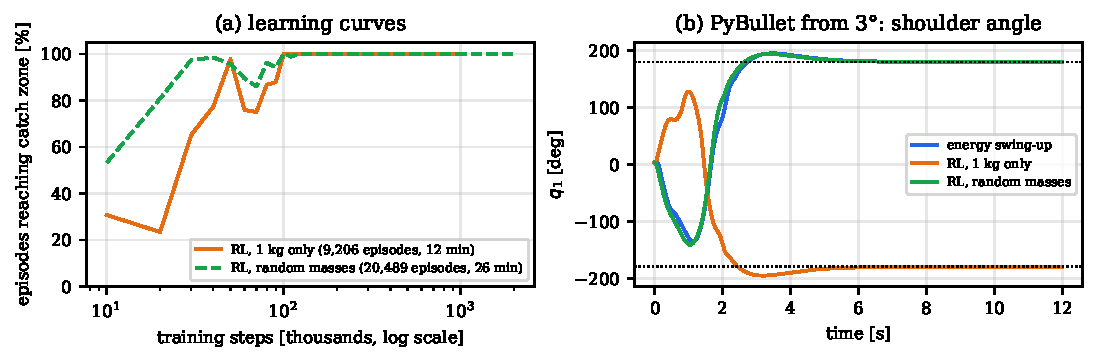
\includegraphics[width=\textwidth]{figures/fig_training.pdf}
\caption{(a) Share of training episodes that reached the catch zone, for the original policy and for the robust policy of Section~\ref{sec:robust} (log scale). (b) PyBullet runs from $3^\circ$: the original RL policy swings the other way and ends at $q_1=-180^\circ$, the same upright pose as $+180^\circ$; the robust policy swings the same way as the energy law.}
\label{fig:training}
\end{figure}
\textbf{Observations:}
\begin{itemize}
\item The policy first reached the catch zone in every episode after about $10^5$ steps (72~s of training) and stayed at 100\% for the remaining $9\times10^5$ steps.
\item Episodes kept getting shorter (more episodes per $10^4$ steps: 54 at $10^5$, 110 at $10^6$): the policy kept learning to reach the top faster.
\item The robust policy (Section~\ref{sec:robust}), which faces a different robot in every episode, also first reached 100\% after about $10^5$ steps. Over its remaining $1.9\times10^6$ steps it never dropped below 98.8\%.
\end{itemize}

\subsection{Results: Correct Model}
Both controllers were tested from the same 40 random starts as Phase~4. A start counts as held if it is caught and balanced within 30~s. (This is why the energy controller scores 35 rather than the Phase~4 value of 39, which allowed 40~s.)
\begin{table}[H]
\centering
\caption{RL vs.\ energy swing-up, correct masses ($|\tau|\le20\Nm$)}
\label{tab:rlnom}
\begin{tabular}{|l|c|c|}
\hline
Metric & Energy swing-up & RL swing-up (SAC)\\ \hline
Held (of 40) & 35 & \textbf{40}\\
Median time to first catch & 3.98 s & \textbf{1.71 s}\\
Time at the torque limit & 8.8\% & \textbf{0.1\%}\\
Median elbow work & 244.9 J & \textbf{144.5 J}\\
PyBullet from $3^\circ$: first catch & 2.17 s & \textbf{1.76 s}\\ \hline
\end{tabular}
\end{table}
\textbf{Observations:}
\begin{itemize}
\item \textbf{Reliability:} RL caught all 40 starts; the energy law caught 35 within 30~s.
\item \textbf{Speed:} RL reaches the top more than twice as fast (median 1.71 s vs.\ 3.98 s).
\item \textbf{Control effort:} RL almost never saturates the motor (0.1\% vs.\ 8.8\%) and uses 41\% less work. In Phase~4 saturation was what broke the energy law; the policy learned a timing that stays within $20\Nm$ by itself.
\end{itemize}

\subsection{Results: Wrong Model}
The real robot never matches the model exactly. The same 40 starts were rerun with both link masses changed by $\pm20\%$ (inertias scaled with them). Both controllers still assume 1~kg links.
\begin{table}[H]
\centering
\caption{Robustness to the link masses (held of 40, within 30 s)}
\label{tab:rlrob}
\begin{tabular}{|l|c|c|}
\hline
Link masses & Energy swing-up & RL swing-up (SAC)\\ \hline
$-20\%$ (0.8 kg) & 37 & 38\\
correct (1.0 kg) & 35 & 40\\
$+20\%$ (1.2 kg) & \textbf{35} & \textbf{15}\\ \hline
\end{tabular}
\end{table}
\begin{itemize}
\item \textbf{The energy law degrades gracefully} (35--37 of 40 in every case). It is built from physics: it pumps until $E=E_{top}$, so a heavier arm just takes a little longer (median 5.4~s instead of 4.0~s).
\item \textbf{RL collapses on heavier links} (15 of 40). It practised only on 1~kg links, so it learned the \emph{timing of that particular robot}, not the physics. It still reaches the catch zone in all 40 runs, but in a state from which the LQR cannot hold the heavier arm; it then repeats nearly the same approach (a median of 13 hand-overs in 30~s instead of 2).
\item \textbf{The fix} is to let the policy practise on many different robots (Section~\ref{sec:robust}).
\end{itemize}

\subsection{Making the Policy Robust}\label{sec:robust}
A second policy was trained with exactly \textbf{two changes}. Everything else (network, reward, catch zone, LQR and SAC settings) is the same, so any difference in the results comes from these two changes.
\begin{table}[H]
\centering
\caption{The two changes for the robust policy}
\label{tab:robustchanges}
\small
\begin{tabular}{|>{\raggedright\arraybackslash}p{2.5cm}|>{\raggedright\arraybackslash}p{3.0cm}|>{\raggedright\arraybackslash}p{4.6cm}|>{\raggedright\arraybackslash}p{4.0cm}|}
\hline
& \textbf{Original policy} & \textbf{Robust policy} & \textbf{Why}\\ \hline
1. Link masses in training & always 1 kg & new random $m_1,m_2\in[0.7,1.3]$ kg in every episode & it cannot memorise one robot's timing\\ \hline
2. Observation & the 6 numbers of Table~\ref{tab:env} & the same 6, plus the missing energy $(E_{top}-E)/E_{top}$ & the quantity the energy law steers by\\ \hline
Training length & $10^6$ steps, 9\,206 episodes, 12.4 min & $2\times10^6$ steps, 20\,489 episodes, 25.9 min & many robots make a harder task\\ \hline
\end{tabular}
\end{table}
The extra input is computed from the other six with the nominal 1~kg model, exactly as the energy controller computes it. It therefore adds no new information: it is a hint that makes the important quantity explicit. Change~1 is the real fix (this is called \emph{domain randomization}). By the end of training the robust policy reached the catch zone in 100\% of episodes, as the original did.

All three swing-ups were then tested from the same 40 starts with five link masses. Two of them (0.6 and 1.4 kg) lie \emph{outside} the range the robust policy practised on. Every controller still assumes 1~kg links.
\begin{table}[H]
\centering
\caption{Held of 40 random starts (within 30 s) for five link masses}
\label{tab:rlrob2}
\resizebox{\textwidth}{!}{\begin{tabular}{|l|c|c|c|}
\hline
True link masses & Energy swing-up & RL, 1 kg only & RL, random masses\\ \hline
0.6 kg ($-40\%$, never practised) & 39 & 2 & \textbf{40}\\
0.8 kg ($-20\%$) & 37 & 38 & \textbf{40}\\
1.0 kg (correct) & 35 & \textbf{40} & \textbf{40}\\
1.2 kg ($+20\%$) & 35 & 15 & \textbf{40}\\
1.4 kg ($+40\%$, never practised) & \textbf{33} & 3 & 2\\ \hline
\end{tabular}}
\end{table}
\begin{figure}[H]
\centering
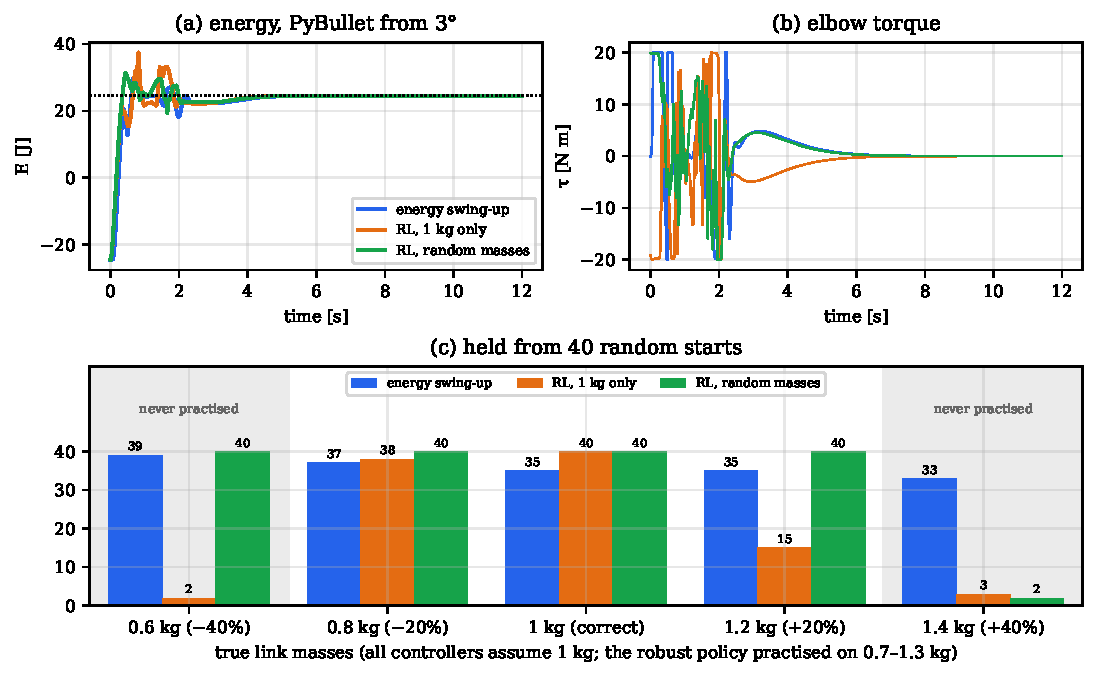
\includegraphics[width=\textwidth]{figures/fig_compare.pdf}
\caption{(a) Energy and (b) elbow torque in PyBullet from $3^\circ$ for the three swing-ups; (c) starts held for five link masses. Shaded: masses the robust policy never practised on.}
\label{fig:compare}
\end{figure}
\textbf{Observations:}
\begin{itemize}
\item \textbf{Inside the practised range the problem is solved:} 40 of 40 at every mass from 0.8 to 1.2~kg. At $+20\%$ the score rises from 15 to 40.
\item \textbf{No price on the correct model:} the robust policy also holds 40 of 40, with the same median catch time (1.71~s), no saturation (0.0\%) and 10\% less elbow work (130.0~J vs.\ 144.5~J). In PyBullet from $3^\circ$ it catches at 1.89~s (original 1.76~s).
\item \textbf{Lighter than ever practised (0.6~kg):} still 40 of 40. The original policy managed only 2, and in 25 of its 40 runs it never even reached the catch zone.
\item \textbf{Much heavier than ever practised (1.4~kg):} only 2 of 40, while the energy law still holds 33. The policy reaches the catch zone in all 40 runs, but the hand-over fails again and again (a median of 12 hand-overs in 30~s, against 1 for the energy law). The energy law also loses many first catches, but each new approach is different, so a later catch usually works; the policy repeats nearly the same approach.
\item \textbf{Why the hand-over is the weak point:} the reward ends the episode as soon as the arm \emph{enters} the catch zone. The policy is never told whether the LQR then holds the arm, so it never learned to deliver the arm in an easy-to-catch state.
\end{itemize}
\textbf{Lesson:} a learned controller is reliable over the variety of robots it practised on (here, also somewhat beyond it on the light side). A physics-based law knows \emph{why} it works, so it extrapolates further. Two natural next steps would be to reward holding rather than only arriving (end each episode only after the LQR has held the arm for, say, 1~s) and to widen the mass range.

\subsection{Discussion}
\begin{enumerate}
\item \textbf{Why RL is faster and gentler.} The energy law fixes the elbow motion through $v$ and pays for it with saturation. The policy is free to choose any torque profile and is rewarded for reaching the top quickly with little effort, so it found a timing that pumps energy faster without hitting the limit.
\item \textbf{Why RL was fragile, and what fixed it.} Its knowledge is implicit in $256\times256$ hidden units fitted to the robots it practised on. Practising on one robot gave that robot's timing; practising on many made it robust over that range. Nothing in it says ``pump until $E=E_{top}$'', however, so far outside that range (1.4~kg) it can still fail where the energy law does not.
\item \textbf{Guarantees.} The LQR catch has a Lyapunov certificate (Phase~3). The learned part has none: its performance is known only from tests, which is why it was tested on 40 starts, in a second simulator (PyBullet) and with five different link masses.
\item \textbf{Hybrid design.} Learning the hard nonlinear part and keeping the provable part near the top gave the best of both: the speed of RL, and a guaranteed final balance.
\end{enumerate}
